%% IMPORTANT NOTICE:
%% 
%% For the copyright see the source file.
%% 
%% For distribution of the original source see the terms
%% for copying and modification in the file samples.dtx.
%% 
%% This generated file may be distributed as long as the
%% original source files, as listed above, are part of the
%% same distribution. (The sources need not necessarily be
%% in the same archive or directory.)
%%
%% The first command in your LaTeX source must be the \documentclass command.
\documentclass[sigchi]{acmart}

%%
%% \BibTeX command to typeset BibTeX logo in the docs
\AtBeginDocument{%
  \providecommand\BibTeX{{%
    \normalfont B\kern-0.5em{\scshape i\kern-0.25em b}\kern-0.8em\TeX}}}

%% Rights management information.  This information is sent to you
%% when you complete the rights form.  These commands have SAMPLE
%% values in them; it is your responsibility as an author to replace
%% the commands and values with those provided to you when you
%% complete the rights form.
\setcopyright{acmcopyright}
\copyrightyear{2019}
\acmYear{2019}
\acmDOI{10.1145/1122445.1122456}

%% These commands are for a PROCEEDINGS abstract or paper.
\acmConference[UbiComp'19]{the ACM Conference on Ubiquitous Computing}{Sept 11--13, 2019}{London, UK}
\acmPrice{15.00}
\acmISBN{978-1-4503-9999-9/18/06}


%%
%% Submission ID.
%% Use this when submitting an article to a sponsored event. You'll
%% receive a unique submission ID from the organizers
%% of the event, and this ID should be used as the parameter to this command.
%%\acmSubmissionID{123-A56-BU3}

%%
%% end of the preamble, start of the body of the document source.
\begin{document}

%%
%% The "title" command has an optional parameter,
%% allowing the author to define a "short title" to be used in page headers.
\title{HiveTracker: 3D Positioning for Ubiquitous Embedded Systems}
%\title{HiveTracker: Embedded 3D Positioning, Algorithms and Characterizations}

%%
%% The "author" command and its associated commands are used to define
%% the authors and their affiliations.
%% Of note is the shared affiliation of the first two authors, and the
%% "authornote" and "authornotemark" commands
%% used to denote shared contribution to the research.
\author{C\'edric Honnet}
%\orcid{1234-5678-9012}
\affiliation{%
  \institution{Sorbonne University, ISIR, CNRS}
  \streetaddress{}
  \city{Paris}
  \country{France}}
\email{cedric@honnet.eu}

\author{Gon\c{c}alo Lopes}
\affiliation{%
  \institution{NeuroGEARS Ltd}
  \streetaddress{}
  \city{London}
  \country{United Kingdom}}
\email{g.lopes@neurogears.org}

\begin{teaserfigure}
\centering
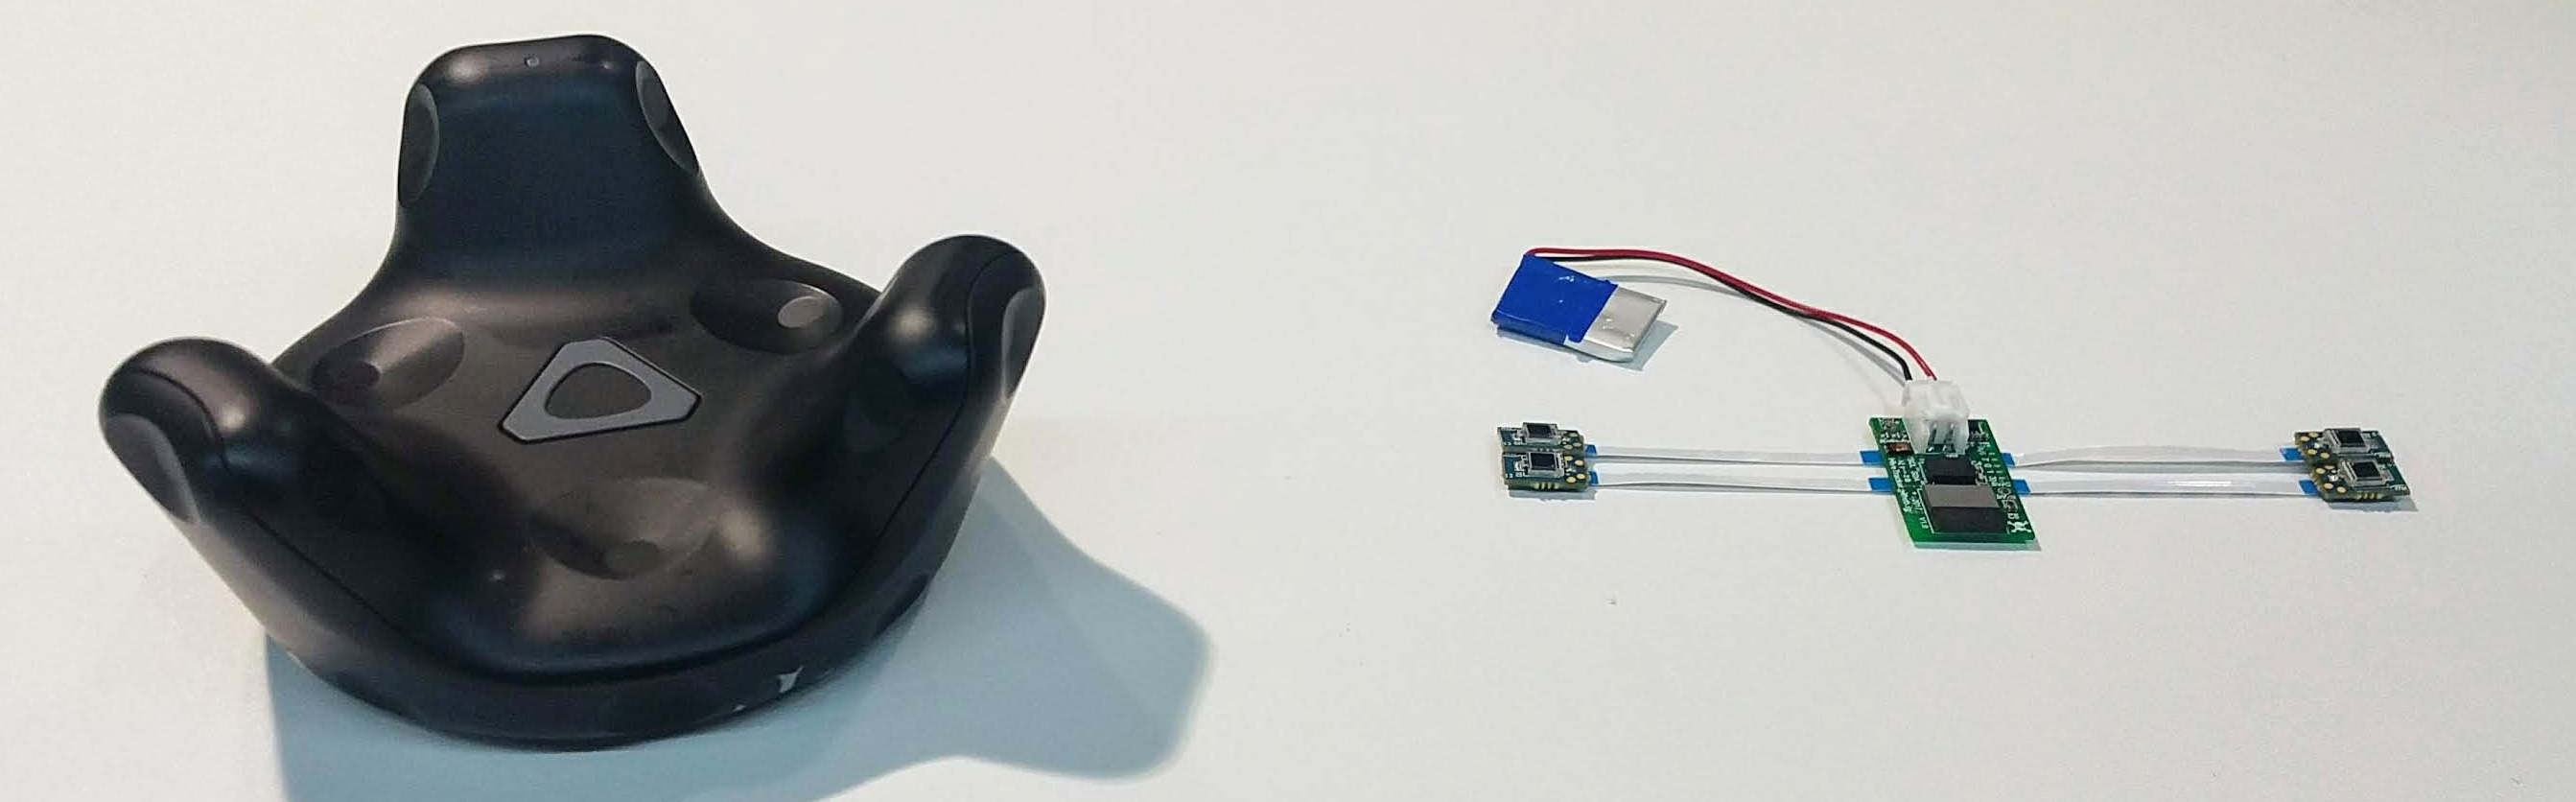
\includegraphics[width=1.0\columnwidth]{Figures/banner.jpg}
\caption{Left: the HTC Vive tracker - Right: our HiveTracker miniaturization.}
\label{Fig:Banner}
\end{teaserfigure}

%%
%% The abstract is a short summary of the work to be presented in the
%% article.
\begin{abstract}
Recent advances in positional tracking systems for virtual and augmented reality have opened up the possibilities for ubiquitous motion capture technology in the consumer market. However, for many applications such as in performance art, athletics, neuroscience, and medicine, these systems remain too bulky, expensive, and limited to tracking a few objects at a time. In this work, we present a small wireless device that takes advantage of existing HTC Vive lighthouse tracking technology to provide affordable, scalable, and highly accurate positional tracking capabilities. This open hardware and open software project contains several elements, and the latest contributions described in this paper include: (1) a characterization of the optical distortions of the lighthouses, (2) a new cross-platform WebBLE interface, and (3) a real-time in-browser visualization. We also introduce the possibility of: (1) a new adaptive calibration using regression to estimate transformation matrices of lighthouses, and (2) an FPGA approach to allow more photodiodes, and to adapt to HTC Vive lighthouses V2. Finally, we show how the new developments reduce setup costs and increase the accessibility of our tracking technology.
\end{abstract}

%%
%% The code below is generated by the tool at http://dl.acm.org/ccs.cfm.
%% Please copy and paste the code instead of the example below.
%%

\begin{CCSXML}
<ccs2012>
<concept>
<concept_id>10003120.10003121.10003125</concept_id>
<concept_desc>Human-centered computing~Interaction devices</concept_desc>
<concept_significance>500</concept_significance>
</concept>
</ccs2012>
\end{CCSXML}

\ccsdesc[500]{Human-centered computing~Interaction devices}


%%
%% Keywords. The author(s) should pick words that accurately describe
%% the work being presented. Separate the keywords with commas.
\keywords{Indoor Positioning, Open-source, Low Cost, Wireless Device, Virtual Reality, 3D Tracking}


%%
%% This command processes the author and affiliation and title
%% information and builds the first part of the formatted document.
\maketitle

%%%%%%%%%%%%%%%%%%%%%%%%%%%%%%%%%%%%%%%%%%%%%%%%%%%%%%%%%%%%%%%%%%%%%%%%%%%%%%%%%%%%%%%%%%%%%%
\section{Introduction}
Robust real-time positional tracking systems have been the target of research for decades to support applications in natural user interfaces (NUI), virtual reality (VR) and augmented reality (AR). All of these interface paradigms require an accurate sampling of the spatial environment of a user, and have to be responsive in real-time in order to sustain the illusion of control. Recent developments in motion sensing and tracking technology for VR have finally moved the field of motion capture technology away from expensive custom engineered spaces with multiple cameras. The need to deploy VR in the consumer market has pushed for scalable and cost-effective solutions, mostly through inside-out computer vision based simultaneous localization and mapping (SLAM) \cite{Klein2007,Whelan2016} or laser-based lighthouse approaches \cite{Borges2018}.
\newline
Because each device is taking care of its own localization, such inside-out solutions are inherently scalable, allowing for a much larger number of devices to coexist in the same space. This has triggered many researchers to start rethinking the entire approach to full-body motion tracking, replacing the passive reflective beads with active inside-out devices \cite{Jiang2016}. Unfortunately, size and accuracy remain a limitation for such motion capture applications. Inside-out SLAM based computer vision devices rely on cameras and expensive processors, which both make existing controllers more bulky and increase power requirements.

An alternative solution to inside-out tracking is to use a beacon-based approach, such as the one used in the HTC Vive Lighthouse tracking system. In this system, a lighthouse base station periodically sweeps the space with a laser at a fixed frequency. Photodiodes placed in tracked objects can detect these sweeps and using either information embedded in modulated light at the beam, or synchronization pulses, can reconstruct the exact angle at which the laser hit the object. Positioning information can be accurately recovered from the photodiodes as long as the timing of each laser hit can be sensed fast enough.


%%%%%%%%%%%%%%%%%%%%%%%%%%%%%%%%%%%%%%%%%%%%%%%%%%%%%%%%%%%%%%%%%%%%%%%%%%%%%%%%%%%%%%%%%%%%%%
\section{Contributions}

In previous work, we introduced the first HiveTracker\footnote{\url{https://hivetracker.github.io}} prototype \cite{Quinones2018}, which takes advantage of a rare dedicated real-time and parallel processing feature in the nRF52 microcontroller made by Nordic Semiconductor to sense the lighthouse light sweeps, without requiring a dedicated FPGA. This allowed us to build an embedded device with up to five photodiodes that is small, accurate, and cheap enough for full-body motion tracking at scale.
\newline \newline
In this paper, we describe the further development of our miniaturized prototype (see Fig. \ref{Fig:Banner}), and the main hardware and software challenges we had to overcome to increase the accessibility and ease of use of the HiveTracker beyond a proof-of-concept.


\subsection{Optical distortion characterization}

To better understand the limitations of our system, we designed a simple test version to characterize it and improve it accordingly.

\subsubsection{Test jig}
The 1st step was to verify that we can measure a coherent 10 mm translation wherever we are in our working zone.
We used a CNC \footnote{XY-plotter by Makeblock: \url{http://www.makeblock.com}} to sample positions along a
linear path. We moved the CNC on 7 locations, and for each of them, we sampled 30 position data every 10mm.
The HTC Vive positioning being accurate with the HTC recommended setup, we explored the limits of its capabilities.
Instead of making the base stations face toward each other, we made them look in the same direction, as
represented in figure \ref{Fig:characterization_jig}.

\begin{figure}[h]
  \centering
  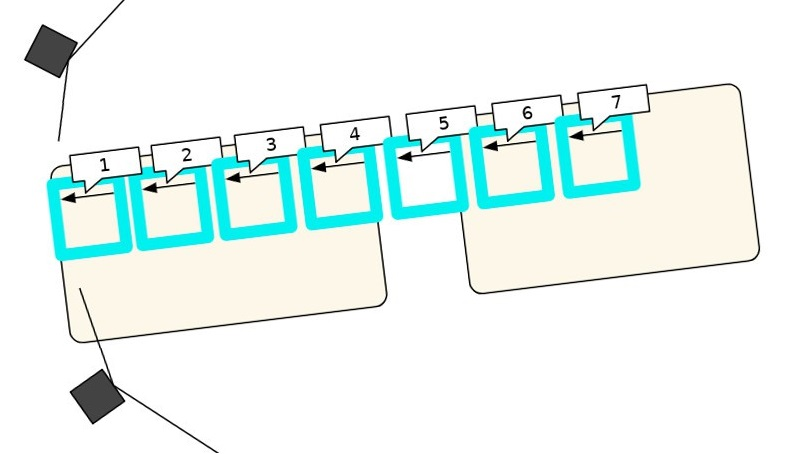
\includegraphics[width=\linewidth]{Figures/characterization_jig.jpg}
  \caption{Characterization jig: each numbered square is a position of the CNC.}
  \label{Fig:characterization_jig}
\end{figure}

\subsubsection{Result}
As we can see in the figure \ref{Fig:characterization_result}, the HTC Vive positioning system is not linear in this configuration. The observed distortion shows that measuring a distance of 300mm near the base stations is not the same as measuring the same distance further away. Nevertheless, now that we have characterized it becomes possible to calibrate a distortion map so we can improve our positioning measurements later.

\begin{figure}[h]
  \centering
  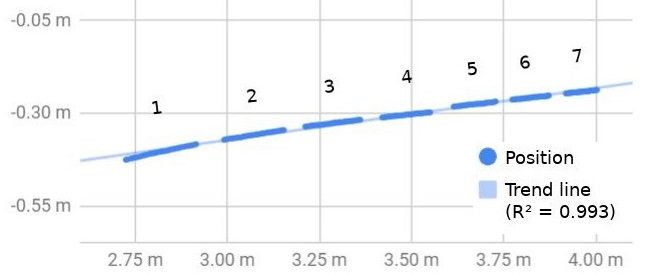
\includegraphics[width=\linewidth]{Figures/characterization_result.jpg}
  \caption{Characterization result: each numbered line is a measurement of a 300mm distance.}
  \label{Fig:characterization_result}
\end{figure}

\subsection{Firmware}

The entire development stack of the project is open source, with the goal of making all components as accessible as possible. For instance, we worked hard to make our firmware\footnote{Firmware Reposiory: \url{http://github.com/hivetracker/firmware}} Arduino compatible. Fortunately, the latest
Arduino "Nano 33 BLE"\footnote{Arduino Nano 33 BLE: \url{https://store.arduino.cc/usa/nano-33-ble}} uses the same microcontroller (nRF52) as our prototype, which will allow us to ensure long term support.

\subsection{Bluetooth Low Energy communication}

The nRF52 microcontroller provides a proprietary radio communication protocol for high-bandwidth communication, but also a BLE interface. BLE communication is attractive due to its low power requirements and growing acceptance as a standard in web development stacks. In our goal to make setting up and interfacing with HiveTracker devices more accessible, we decided to embed a lightweight BLE protocol in the device firmware, allowing direct pairing from any WebBLE enabled browser.

As mentioned in the previous section, all our tools are chosen with the goal of making the project accessible and reproducible. Up to now WebBLE was the most easily accessible route for reading BLE data streams, but alternative approaches have been recently published by the ITP-NYU community: p5.ble.js\footnote{p5.ble.js by ITP-NYU: \url{https://ItpNyu.github.io/p5ble-website/}}. These should hopefully help improve the accessibility of this project further.


\subsection{Real-time visualization in a web app}

To enable rapid-prototyping, visualization and testing of the HiveTracker performance, we developed an in-browser JavaScript interface, visualization and simulation framework using the Three.js library\footnote{Three.js library: \url{https://threejs.org/}}. This cross-platform approach allows visualizing the 3D positions in any device running Chromium or Chrome (see figure \ref{Fig:webapp}). This interface can be tested, and modified from our repository \footnote{Web app Repository: \url{http://github.com/hivetracker/hivetrackerjs}}. This will enable mobile applications such as smartphone web apps for motion capture or augmented reality.

\begin{figure}[h]
  \centering
  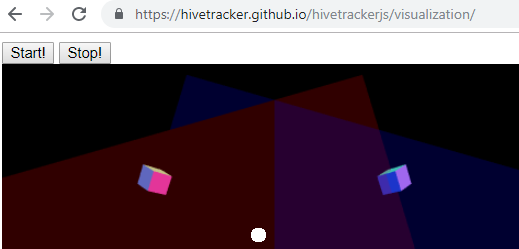
\includegraphics[width=\linewidth]{Figures/webapp.png}
  \caption{Web app showing the 2 base stations (cubes) and the tracker (sphere).}
  \label{Fig:webapp}
\end{figure}


%%%%%%%%%%%%%%%%%%%%%%%%%%%%%%%%%%%%%%%%%%%%%%%%%%%%%%%%%%%%%%%%%%%%%%%%%%%%%%%%%%%%%%%%%%%%%%
\section{Future work}

\subsection{3D reconstruction and adaptive calibration}

For each photodiode laser hit, we can reconstruct the positioning information of the sensor relative to the origin of the base station. However, it is often desirable to position the device relative to a common reference frame. In our previous work \cite{Quinones2018}, we directly used the SteamVR calibration procedure to extract the location of each base station in absolute VR world coordinates. This was useful when integrating with existing VR applications running on the computer, for example to keep the coordinate frame of the device registered with a VR headset. However, the base station beacons are completely passive and only require a power supply, so it would also be an advantage to allow the calibration of a common reference frame independent of SteamVR, for situations where we are running a motion capture system in full-wireless mode, independently from a computer.

To calibrate our own reference, we use a HiveTracker device as the origin, with four photodiodes arranged in a known planar configuration (see figure \ref{Fig:squared_structure}).

\begin{figure}[h]
  \centering
  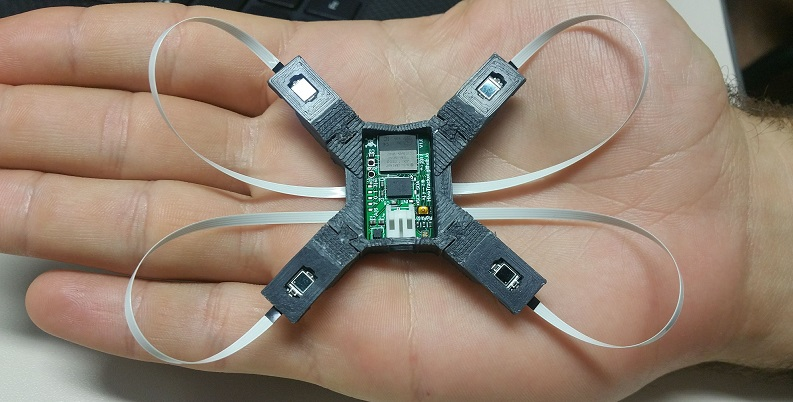
\includegraphics[width=\linewidth]{Figures/squared_structure.jpg}
  \caption{Squared structure used for calibration.}
  \label{Fig:squared_structure}
\end{figure}

For each pair of photodiode hits from the same base station, we recover two angles, from which we can reconstruct the line from the photodiode to the origin of each base station (Figure \ref{Fig:Reconstruction}A). By projecting each line onto a fixed distance plane in front of the beacon, we recover 2D positions of points at the surface of the beacon plane (Figure \ref{Fig:Reconstruction}B). Given we also know, by definition, the 3D coordinates of each of these points on the origin device, we can fully define a set of 2D/3D correspondences ($N = 4$). This is an instance of the well-known Perspective-N-Point problem for planar fiducial markers, for which there are a number of efficient solutions \cite{Lepetit2008,Garrido-Jurado2014}. After independently computing the pose of the origin device relative to both beacons, we can make use of bundle adjustment methods such as the Levenberg-Marquardt algorithm \cite{Marquardt1963} to further improve the overall estimate of the beacon poses relative to the origin. In principle, we could extend this procedure to a grid of devices to further improve the estimated quality, as in \cite{Garrido-Jurado2014}.

\begin{figure}[h]
\centering
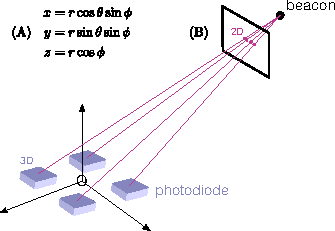
\includegraphics[width=1.0\columnwidth]{Figures/reconstruction.pdf}
\caption{Schematic of reconstruction procedure. (A): Relation of polar coordinates to cartesian coordinates, where $\theta$ and $\phi$ are the angles recovered from the device. (B): Projection of angles into fixed distance plane to generate 2D/3D correspondences.}
\label{Fig:Reconstruction}
\end{figure}


\subsection{Hardware improvements using FPGAs}

Until now, we focused on keeping the hardware\footnote{\url{https://upverter.com/profile/hivetracker/}} simple, affordable, and scalable. However, a new version of the HTC LightHouse has been released which brings new features that both reduce the cost of basestations and enable for a larger tracking range using multiple beacons. This new version introduces the need for a very different sensing architecture using modulated light. Our nRF52 approach is not suitable for this, so we will need to redesign our sensing hardware to use an FPGA. Fortunately, some FPGAs have been released which are both very small and well supported by the open source community\footnote{Open Software FPGA Toolchain: \url{http://clifford.at/IceStorm}} such as the Lattice iCE40UL-1K. Its 1.4mm x 1.4mm package allows us to stay compact, and to support more photodiodes.


%%%%%%%%%%%%%%%%%%%%%%%%%%%%%%%%%%%%%%%%%%%%%%%%%%%%%%%%%%%%%%%%%%%%%%%%%%%%%%%%%%%%%%%%%%%%%%
\section{Conclusion}

In this work, we presented a new scalable wireless 3D tracking device that we believe has the potential to open up new possibilities in the field of motion capture and behaviour studies, athletics performance, art, and medical diagnosis. The main motivation was to develop the entire stack of hardware and software on top of open and accessible standards, with the goal of maximizing dissemination of this state-of-the-art technology. The challenges have been numerous, and while much work remains to be done, here we showed that all of the remaining steps are dependent on current, immediately available technology. Our goal with this publication is to inspire others to join our development journey.

%%
%% The acknowledgments section is defined using the "acks" environment
%% (and NOT an unnumbered section). This ensures the proper
%% identification of the section in the article metadata, and the
%% consistent spelling of the heading.
\begin{acks}
The authors would like to thank Adam Kampff, Yvonne Jansen and Alexis Polti for their support offered during the development of this project. We would also like to thank Julien Mellet for his early work on reconstruction algorithms, Chinmay Pendharkar for his vital WebBLE contribution, Olivia Seow and Chris Davis for their design and media expertise, and NeuroGEARS Ltd. for the financial support as well as the provided help. This project was partially funded by the "Human Computer Interface Prize" of the Hack-A-Day conference. Finally, this work was also partially performed within the Labex SMART (ANR-11-LABX-65), supported by French state funds managed by the ANR under reference ANR-11-IDEX-0004-02.
\end{acks}

%%
%% The next two lines define the bibliography style to be used, and
%% the bibliography file.
\bibliographystyle{ACM-Reference-Format}
\bibliography{ubicomp-2019}

%%
%% If your work has an appendix, this is the place to put it.
%\appendix

\end{document}
\endinput
%%
%% End of file `sample-sigchi.tex'.
